
\section{Scale-up Server Scalability}
\label{sec:scale}




%$$$$$$$$$$$$$$$$$$$$$$$$$$$$$$$$$$$$$$$$$$$$$$$$$$$$$$$$$$$$$$$$$$$$$$$$$$$$$$$$
%$$$$$$$$$$$$$$$$$$$$$$$$$$$$$$$$$$$$$$$$$$$$$$$$$$$$$$$$$$$$$$$$$$$$$$$$$$$$$$$$
% 이번 장에 대한 설명
%$$$$$$$$$$$$$$$$$$$$$$$$$$$$$$$$$$$$$$$$$$$$$$$$$$$$$$$$$$$$$$$$$$$$$$$$$$$$$$$$
\ifkor
\else

\fi



\subsection{Test-bed and Benchmark}

%$$$$$$$$$$$$$$$$$$$$$$$$$$$$$$$$$$$$$$$$$$$$$$$$$$$$$$$$$$$$$$$$$$$$$$$$$$$$$$$$
%$$$$$$$$$$$$$$$$$$$$$$$$$$$$$$$$$$$$$$$$$$$$$$$$$$$$$$$$$$$$$$$$$$$$$$$$$$$$$$$$
% Apache Spark에 대한 설명
%$$$$$$$$$$$$$$$$$$$$$$$$$$$$$$$$$$$$$$$$$$$$$$$$$$$$$$$$$$$$$$$$$$$$$$$$$$$$$$$$
\ifkor
\noindent
\textbf{Apache Spark. }
Apache Spark is a framework for large scale distributed computation.
RDD(Resilient Distributed Datasets) is a collection of partitions of records, 
and the RDD is managed as LRU(Least Recently Used), so when there is not enough
memory, Spark evicts the least recently used RDD.
Spark may has a substantial performance when data-set can fit in memory.

%\begin{figure}[h]
%    \centering
%    \begin{subfigure}[b]{0.22\textwidth}
%        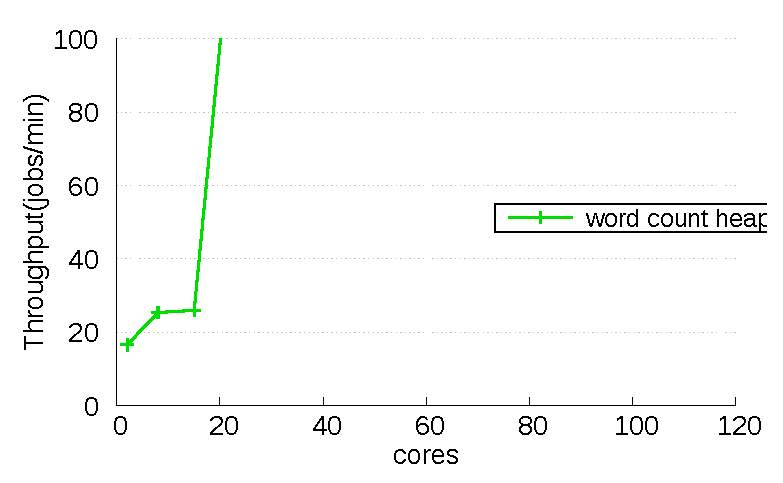
\includegraphics[width=1.5in]{graph/wc_max.eps}
%        \caption{Word Count}
%    \end{subfigure}%
%    \begin{subfigure}[b]{0.22\textwidth}
%        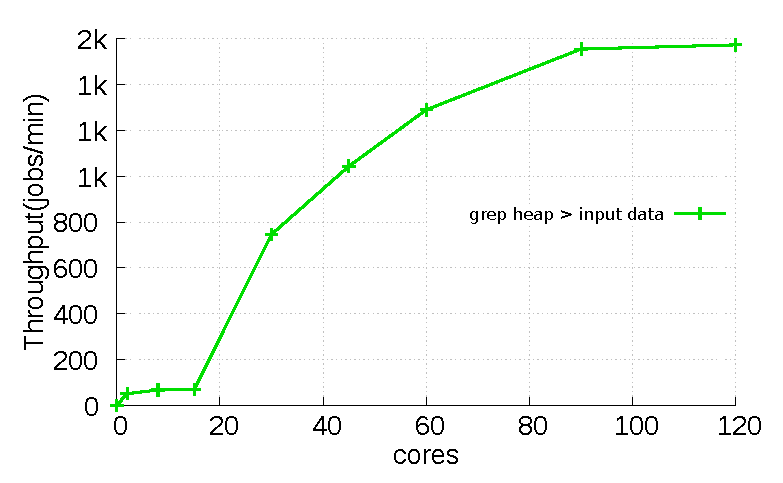
\includegraphics[width=1.5in]{graph/grep_max.eps}
%        \caption{Grep}
%    \end{subfigure}
%    \caption{CPU utilization on 120 core.}
%    \label{fig:utilization}
%\end{figure}

%Figure shows a substantial performance scalability of Spark when dataset can
% fit in memory(heap size > data size).
%However, large scale data(head size < data size) does not scale on scale-up
%server due to the GC and the memory latency.
\else
\fi

%$$$$$$$$$$$$$$$$$$$$$$$$$$$$$$$$$$$$$$$$$$$$$$$$$$$$$$$$$$$$$$$$$$$$$$$$$$$$$$$$
%$$$$$$$$$$$$$$$$$$$$$$$$$$$$$$$$$$$$$$$$$$$$$$$$$$$$$$$$$$$$$$$$$$$$$$$$$$$$$$$$
% 테스트 베드 설명
%$$$$$$$$$$$$$$$$$$$$$$$$$$$$$$$$$$$$$$$$$$$$$$$$$$$$$$$$$$$$$$$$$$$$$$$$$$$$$$$$
\ifkor
\noindent
\textbf{Test-bed. }
We use a machine to evaluate on real hardware: an 120-core (8 sockets × 15
cores) Intel Xeon E7-8870 (the same machine used for evaluation in chapter X)
and, to show that our conclusions generalize.
Hyper-Threading is disabled, and we used Linux kernel 4.5-rc6.

\begin{figure}[h]
  \begin{center}
     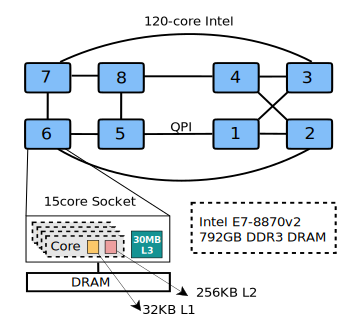
\includegraphics[width=0.3\textwidth]{fig/xeon}
  \end{center}
  \caption{Test-bed intel xeon archtecture.}
  \label{fig:basic}
\end{figure}
\else

\fi

%$$$$$$$$$$$$$$$$$$$$$$$$$$$$$$$$$$$$$$$$$$$$$$$$$$$$$$$$$$$$$$$$$$$$$$$$$$$$$$$$
%$$$$$$$$$$$$$$$$$$$$$$$$$$$$$$$$$$$$$$$$$$$$$$$$$$$$$$$$$$$$$$$$$$$$$$$$$$$$$$$$
%Benchamrk에 대한 설명
%$$$$$$$$$$$$$$$$$$$$$$$$$$$$$$$$$$$$$$$$$$$$$$$$$$$$$$$$$$$$$$$$$$$$$$$$$$$$$$$$
\noindent
\textbf{Benchmark.} We used BigData Benchmark.

\begin{table}[h!]
  \centering
  \small
  \begin{tabular}{l r r r r} \toprule
    workload & input data size & heap size & configuration \\
    \midrule
    Word Count & 2487 s & 1993 s & 4647 s(51\%)\\ 
    Naive Basian & 1123 s & 3631 s & 2186 s(31\%)\\
    Grep & 3630 s & 2511 s & 1466 s(19\%)\\
    K-means & 3630 s & 1903 s & 1662 s(23\%)\\
    \bottomrule
  \end{tabular}
  \begin{tabular}{l r r r r} \toprule
    JVM & BigDataBench & Spark & Hadoop & OS \\
    \midrule
    Jvm 1.8 & BigDataBench & Spark 1.2 & Hadoop & Linux 4.5rc6 \\ 
    \bottomrule
  \end{tabular}

  \caption{Comparison of user, system and idle time at 120 cores.}
  \label{tab:memuse}
\end{table}

%\begin{itemize}
%\item \textbf{Word Count. }We have developed a novel lightweight log-based
%structures with efficient log management implementation.
%\item \textbf{Grep. }
%We applied the in Linux kernel to two reverse mapping(anonymous, file) on
%Our design improved throughput and execution time from 1.5x through 2.7x on 120
% core.
%\item \textbf{Naive Basian. }
%We applied the in Linux kernel to two reverse mapping(anonymous, file) on
%Our design improved throughput and execution time from 1.5x through 2.7x on 120
% core.
%\item \textbf{K-means.}
%We applied the in Linux kernel to two reverse mapping(anonymous, file) on
%Our design improved throughput and execution time from 1.5x through 2.7x on 120
% core.
%\end{itemize}


\subsection{Spark Scalability Problem}
%$$$$$$$$$$$$$$$$$$$$$$$$$$$$$$$$$$$$$$$$$$$$$$$$$$$$$$$$$$$$$$$$$$$$$$$$$$$$$$$$
%$$$$$$$$$$$$$$$$$$$$$$$$$$$$$$$$$$$$$$$$$$$$$$$$$$$$$$$$$$$$$$$$$$$$$$$$$$$$$$$$
%Scalability 결과에 대한 대략 적인 설명
%$$$$$$$$$$$$$$$$$$$$$$$$$$$$$$$$$$$$$$$$$$$$$$$$$$$$$$$$$$$$$$$$$$$$$$$$$$$$$$$$
Figure 1 shows the Spark scalability of five workloads with two state of the art garbage
collection, G1 and Parallel Scavenge(PS).
Up to 60 core, the five workloads scales lineally and then GC pause becomes bottlenecks.
The Word Count workload flattens out after 60 core, and other benchmarks slightly go
down because not only the GC but also the remote memory access overheads. 
To evaluate state of the art GC, we compared the G1 and PS GC.
The effect of changing to the GC is the PS outperforms G1 by 3.3x on 120 core.
However, although we used the state of the art scalable GC,
the Spark performance scalability still suffers from GC and NUMA locality problem.

%$$$$$$$$$$$$$$$$$$$$$$$$$$$$$$$$$$$$$$$$$$$$$$$$$$$$$$$$$$$$$$$$$$$$$$$$$$$$$$$$
%$$$$$$$$$$$$$$$$$$$$$$$$$$$$$$$$$$$$$$$$$$$$$$$$$$$$$$$$$$$$$$$$$$$$$$$$$$$$$$$$
%CPU utilization에 대한 설명
%$$$$$$$$$$$$$$$$$$$$$$$$$$$$$$$$$$$$$$$$$$$$$$$$$$$$$$$$$$$$$$$$$$$$$$$$$$$$$$$$

Our goal is to maximize CPU utilization, so we profiled the CPU utilization of five workloads.
Figure ~\ref{fig:cpuutilization} shows the CPU utilization.
Th y-axis is the percentage of time spent in kernel-space code(sys), user-space
code(user), and idle time(idle).
All benchmarks increase the idle time due to the GC pause as core counts increase.

%$$$$$$$$$$$$$$$$$$$$$$$$$$$$$$$$$$$$$$$$$$$$$$$$$$$$$$$$$$$$$$$$$$$$$$$$$$$$$$$$
%$$$$$$$$$$$$$$$$$$$$$$$$$$$$$$$$$$$$$$$$$$$$$$$$$$$$$$$$$$$$$$$$$$$$$$$$$$$$$$$$
% Linux kernel scalability (lock, cache cohearnci, scheduler)등등 OS 노이즈에 대한 설명
%$$$$$$$$$$$$$$$$$$$$$$$$$$$$$$$$$$$$$$$$$$$$$$$$$$$$$$$$$$$$$$$$$$$$$$$$$$$$$$$$
\ifkor
%NUMA의 영향 뿐만 아니라, 추가적으로 operating system의 scalability 저해 요소 때문에 
%파티션닝 방법은 필요하다.
%우리는 operation system에서 scalability의 영향을 주는 것을 확인하기 위해 가장먼저
%lock을 조사해보았다.
%첫째로 공유 데이터를 lock이 있다. 표 xxx 앞에서 실험한 spark의 wordcount에 대해서 .
%JVM 위에서 동작하는 thread간의 공유하는 single address space때문에 발생하는 공유 문제이다.
%다음으로 scheduler가 아직 
%마지막으로 cache cohearci traffic이 있다. 
\else

\fi



\subsection{Benefit of JVM Partitioning}
%\subsection{NUMA}

%$$$$$$$$$$$$$$$$$$$$$$$$$$$$$$$$$$$$$$$$$$$$$$$$$$$$$$$$$$$$$$$$$$$$$$$$$$$$$$$$
%$$$$$$$$$$$$$$$$$$$$$$$$$$$$$$$$$$$$$$$$$$$$$$$$$$$$$$$$$$$$$$$$$$$$$$$$$$$$$$$$
%NUMA 영향에 대한 대략 적인 설명
%$$$$$$$$$$$$$$$$$$$$$$$$$$$$$$$$$$$$$$$$$$$$$$$$$$$$$$$$$$$$$$$$$$$$$$$$$$$$$$$$

Spark and Hadoop frameworks use JAVA, and it needs java virtual machine(JVM), so
understanding the partitioning is important.
To preliminarily analyse the JVM partitioning effect, we conducted
benchmarking by using SPECjbb2013~\cite{Pogue2014SO}, which is a state of the art
benchmark for JVM performance.
We used two different experimental settings. 
First, we used per-socket JVM partitioning by using the NUMA control application(numactl).
Second, we set maximum JVM heap size, which is system
available memory size, and threads are scheduled by the OS
in order to migrate any core, and we enable automatic NUMA balancing feature
in the Linux kernel.

\begin{figure}[h]
  \begin{center}
     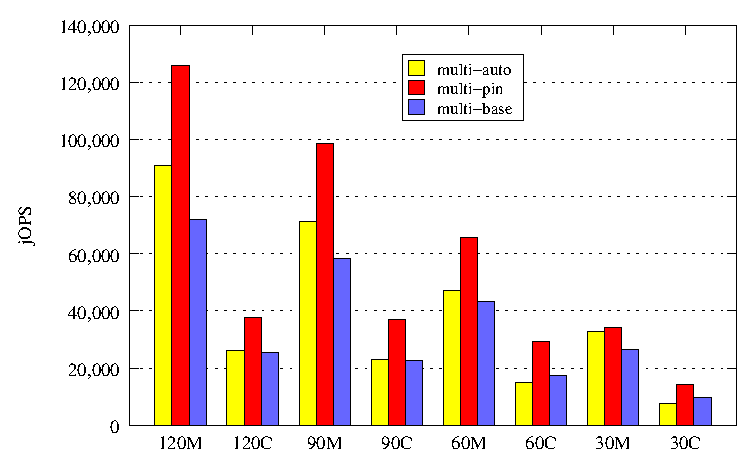
\includegraphics[width=0.4\textwidth]{graph/SPECjbb2013}
  \end{center}
  \caption{Test-bed Intel xeon architecture.}
  \label{fig:basic}
\end{figure}

The results shows that partitioning approach outperforms non-partitioning approach by Xx on 120 core.
Therefore, in manycore scale-up server, partitioning approach has many
advantages over non-partitioning approach in terms of performance scalability.